\documentclass[
  shownotes,
  xcolor={svgnames},
  hyperref={colorlinks,citecolor=DarkBlue,linkcolor=Black,urlcolor=DarkBlue}
  , aspectratio=169]{beamer}
\usepackage{animate}
\usepackage{amsmath}
\usepackage{amsfonts}
\usepackage{amssymb}
\usepackage{pifont}
\usepackage{mathpazo}
%\usepackage{xcolor}
\usepackage{multimedia}
\usepackage{fancybox}
\usepackage[para]{threeparttable}
\usepackage{multirow}
\setcounter{MaxMatrixCols}{30}
\usepackage{subcaption}
\usepackage{graphicx}
\usepackage{lscape}
\usepackage[compatibility=false,font=small]{caption}
\usepackage{booktabs}
\usepackage{ragged2e}
\usepackage{chronosys}
\usepackage{appendixnumberbeamer}
\usepackage{animate}
\setbeamertemplate{caption}[numbered]
\usepackage{color}
%\usepackage{times}
\usepackage{tikz}
\usetikzlibrary{arrows}
\usepackage{comment} %to comment
%% BibTeX settings
\usepackage{natbib}
\bibliographystyle{apalike}
\bibpunct{(}{)}{,}{a}{,}{,}
\setbeamertemplate{bibliography item}{[\theenumiv]}

% Defines columns for bespoke tables
\usepackage{array}
\newcolumntype{L}[1]{>{\raggedright\let\newline\\\arraybackslash\hspace{0pt}}m{#1}}
\newcolumntype{C}[1]{>{\centering\let\newline\\\arraybackslash\hspace{0pt}}m{#1}}
\newcolumntype{R}[1]{>{\raggedleft\let\newline\\\arraybackslash\hspace{0pt}}m{#1}}


\usepackage{xfrac}


\usepackage{multicol}
\setlength{\columnsep}{0.5cm}

% Theme and colors
\usetheme{Boadilla}

% I define a custom pallete
\definecolor{andesred}{HTML}{1B175E}
\definecolor{andesyellow}{HTML}{435982}

% Other options
\providecommand{\U}[1]{\protect\rule{.1in}{.1in}}
\usefonttheme{serif}
\setbeamertemplate{itemize items}[default]
\setbeamertemplate{enumerate items}[square]
\setbeamertemplate{section in toc}[circle]


\definecolor{mybackground}{HTML}{1B175E}
\definecolor{myforeground}{HTML}{0000A0}

\setbeamercolor{normal text}{fg=black,bg=white}
\setbeamercolor{alerted text}{fg=andesred}
\setbeamercolor{example text}{fg=black}

\setbeamercolor{background canvas}{fg=myforeground, bg=white}
\setbeamercolor{background}{fg=myforeground, bg=mybackground}
\setbeamercolor{palette tertiary}{fg=myforeground,bg=mybackground}

\setbeamercolor{palette primary}{fg=black, bg=white}
\setbeamercolor{palette secondary}{fg=black, bg=white!10!andesyellow}
\setbeamercolor{palette tertiary}{fg=black, bg=white}


\setbeamercolor{frametitle}{fg=black}
\setbeamercolor{title}{fg=black}
\setbeamercolor{block title}{fg=andesred}
\setbeamercolor{itemize item}{fg=andesred}
\setbeamercolor{itemize subitem}{fg=andesred}
\setbeamercolor{itemize subsubitem}{fg=andesred}
\setbeamercolor{enumerate item}{fg=andesred}
\setbeamercolor{item projected}{bg=gray!30!white,fg=andesred}
\setbeamercolor{enumerate subitem}{fg=andesred}
\setbeamercolor{section number projected}{bg=gray!30!white,fg=andesred}
\setbeamercolor{section in toc}{fg=andesred}
\setbeamercolor{caption name}{fg=andesred}
\setbeamercolor{button}{bg=gray!30!white,fg=andesred}
\setbeamercolor{title in head/foot}{fg=andesred}



\usepackage{fancyvrb}
\newcommand{\VerbBar}{|}
\newcommand{\VERB}{\Verb[commandchars=\\\{\}]}
\DefineVerbatimEnvironment{Highlighting}{Verbatim}{commandchars=\\\{\}}
% Add ',fontsize=\small' for more characters per line
\usepackage{framed}
\definecolor{shadecolor}{RGB}{248,248,248}
\newenvironment{Shaded}{\begin{snugshade}}{\end{snugshade}}
\newcommand{\AlertTok}[1]{\textcolor[rgb]{0.94,0.16,0.16}{#1}}
\newcommand{\AnnotationTok}[1]{\textcolor[rgb]{0.56,0.35,0.01}{\textbf{\textit{#1}}}}
\newcommand{\AttributeTok}[1]{\textcolor[rgb]{0.77,0.63,0.00}{#1}}
\newcommand{\BaseNTok}[1]{\textcolor[rgb]{0.00,0.00,0.81}{#1}}
\newcommand{\BuiltInTok}[1]{#1}
\newcommand{\CharTok}[1]{\textcolor[rgb]{0.31,0.60,0.02}{#1}}
\newcommand{\CommentTok}[1]{\textcolor[rgb]{0.56,0.35,0.01}{\textit{#1}}}
\newcommand{\CommentVarTok}[1]{\textcolor[rgb]{0.56,0.35,0.01}{\textbf{\textit{#1}}}}
\newcommand{\ConstantTok}[1]{\textcolor[rgb]{0.00,0.00,0.00}{#1}}
\newcommand{\ControlFlowTok}[1]{\textcolor[rgb]{0.13,0.29,0.53}{\textbf{#1}}}
\newcommand{\DataTypeTok}[1]{\textcolor[rgb]{0.13,0.29,0.53}{#1}}
\newcommand{\DecValTok}[1]{\textcolor[rgb]{0.00,0.00,0.81}{#1}}
\newcommand{\DocumentationTok}[1]{\textcolor[rgb]{0.56,0.35,0.01}{\textbf{\textit{#1}}}}
\newcommand{\ErrorTok}[1]{\textcolor[rgb]{0.64,0.00,0.00}{\textbf{#1}}}
\newcommand{\ExtensionTok}[1]{#1}
\newcommand{\FloatTok}[1]{\textcolor[rgb]{0.00,0.00,0.81}{#1}}
\newcommand{\FunctionTok}[1]{\textcolor[rgb]{0.00,0.00,0.00}{#1}}
\newcommand{\ImportTok}[1]{#1}
\newcommand{\InformationTok}[1]{\textcolor[rgb]{0.56,0.35,0.01}{\textbf{\textit{#1}}}}
\newcommand{\KeywordTok}[1]{\textcolor[rgb]{0.13,0.29,0.53}{\textbf{#1}}}
\newcommand{\NormalTok}[1]{#1}
\newcommand{\OperatorTok}[1]{\textcolor[rgb]{0.81,0.36,0.00}{\textbf{#1}}}
\newcommand{\OtherTok}[1]{\textcolor[rgb]{0.56,0.35,0.01}{#1}}
\newcommand{\PreprocessorTok}[1]{\textcolor[rgb]{0.56,0.35,0.01}{\textit{#1}}}
\newcommand{\RegionMarkerTok}[1]{#1}
\newcommand{\SpecialCharTok}[1]{\textcolor[rgb]{0.00,0.00,0.00}{#1}}
\newcommand{\SpecialStringTok}[1]{\textcolor[rgb]{0.31,0.60,0.02}{#1}}
\newcommand{\StringTok}[1]{\textcolor[rgb]{0.31,0.60,0.02}{#1}}
\newcommand{\VariableTok}[1]{\textcolor[rgb]{0.00,0.00,0.00}{#1}}
\newcommand{\VerbatimStringTok}[1]{\textcolor[rgb]{0.31,0.60,0.02}{#1}}
\newcommand{\WarningTok}[1]{\textcolor[rgb]{0.56,0.35,0.01}{\textbf{\textit{#1}}}}
\usepackage{graphicx}
\makeatletter


% colors
\definecolor{airforceblue}{rgb}{0.36, 0.54, 0.66}
\newcommand{\theme}{\color{andesred}}
\newcommand{\bk}{\color{black}}
\newcommand{\rd}{\color{red}}
\newcommand{\fg}{\color{ForestGreen}}
\newcommand{\bl}{\color{blue}}
\newcommand{\gr}{\color{black!60}}
\newcommand{\sg}{\color{DarkSlateGray}}
\newcommand{\br}{\color{SaddleBrown}}
\newcommand{\nv}{\color{Navy}}


% common math markups
\newcommand{\bs}[1]{\boldsymbol{#1}}
\newcommand{\mc}[1]{\mathcal{#1}}
\newcommand{\mr}[1]{\mathrm{#1}}
\newcommand{\bm}[1]{\mathbf{#1}}
\newcommand{\ds}[1]{\mathds{#1}}
\newcommand{\indep}{\perp\!\!\!\perp}

% shorthand
\newcommand{\sk}{\vspace{.5cm}}
\newcommand{\R}[1]{{\tt \nv #1}}
\newcommand{\til}{{\footnotesize$\bs{\stackrel{\sim}{}}$}}
\DeclareSymbolFont{extraup}{U}{zavm}{m}{n}
\DeclareMathSymbol{\vardiamond}{\mathalpha}{extraup}{87}


\usepackage{tikz}
% Tikz settings optimized for causal graphs.
\usetikzlibrary{shapes,decorations,arrows,calc,arrows.meta,fit,positioning}
\tikzset{
    -Latex,auto,node distance =1 cm and 1 cm,semithick,
    state/.style ={ellipse, draw, minimum width = 0.7 cm},
    point/.style = {circle, draw, inner sep=0.04cm,fill,node contents={}},
    bidirected/.style={Latex-Latex,dashed},
    el/.style = {inner sep=2pt, align=left, sloped}
}


\makeatother









\AtBeginSection[]
{
    \begin{frame}
        \frametitle{Agenda}
        \tableofcontents[currentsection]
    \end{frame}
}



\AtBeginSubsection[]
{
    \begin{frame}
        \frametitle{Agenda}
        \tableofcontents[currentsubsection]
    \end{frame}
}




%%%%%%%%%%%%%%% BEGINS DOCUMENT %%%%%%%%%%%%%%%%%%

\begin{document}

\title[MLAM]{¿Qué son los Sistemas de Recomendación?}

\date{}

\author[Sarmiento-Barbieri]{Ignacio Sarmiento-Barbieri}
\institute[Uniandes]{Universidad de los Andes}



\begin{frame}[noframenumbering]
\maketitle
\end{frame}
    
%----------------------------------------------------------------------%
\section{Sobre el curso}

%----------------------------------------------------------------------%
\begin{frame}
\frametitle{Sobre el curso}

\begin{itemize}
    \item Profes:
      \medskip
    \begin{itemize}
    \item Ignacio Sarmiento-Barbieri (i.sarmiento [at] uniandes.edu.co)
    \medskip
    \item Carlos Andrés Rodríguez Bayona (crodriguezbayo [at] uniandes.edu.co)
    
    \end{itemize}
    \medskip
\item Clases: teoría + práctica en \texttt{Python} via  \texttt{Google Colab} 
\medskip
\item Materiales en página web \url{https://ignaciomsarmiento.github.io/teaching/MLAM}
\medskip

\item Certificado de participación a los estudiantes que cursen como mínimo el 85\% de las sesiones (9/10)

\end{itemize}
\end{frame}
%----------------------------------------------------------------------%
\begin{frame}
\frametitle{Sobre el curso}
\framesubtitle{Un poco sobre ustedes}
\begin{itemize}
    
    
        \item Su nombre
        \medskip
        \item En que trabaja
        \medskip
        \item ¿Qué lo motivó a hacer este curso?
            \medskip
        \item ¿Qué espera obtener del curso?
           \medskip
        \item ¿Cuánto conoce de Machine Learning y de Python?
    
    
    

\end{itemize}

\end{frame}
%----------------------------------------------------------------------%
\section{Contenido}
\subsection{Segmentación y arquetipado de consumidores y clientes}
\subsection{Sistemas de recomendación}
%----------------------------------------------------------------------%
\begin{frame}
\frametitle{¿Qué son los sistemas de recomendación?}


\begin{itemize}
    \item ¿Cómo pueden  los usuarios encontrar nuevo contenido/productos atractivos?
    \medskip
    \item Las preferencias siguen patrones que los sistemas de recomendación pueden aprovechar
    \medskip
    \item Los sistemas de recomendación  encuentran patrones para generar sugerencias

    \medskip
    \end{itemize}    
    

\end{frame}
    
    
%----------------------------------------------------------------------%
\begin{frame}
\frametitle{¿Qué son los sistemas de recomendación?}

Los sistemas de recomendación constan principalmente de 2 componentes:
\medskip

\begin{itemize}
    \item Generación de candidatos
    \medskip
    \item Ranking o Puntuación
\end{itemize}

\end{frame}
%----------------------------------------------------------------------%    
\subsubsection{Tipos de sistemas de recomendación}
%----------------------------------------------------------------------%
\begin{frame}
\frametitle{Tipos de sistemas de recomendación}


\begin{itemize}
\item Recomendadores basados en conocimiento
\medskip
\item Filtrado colaborativo
\medskip
\item Filtrado basado en contenido
\medskip
\item Recomendadores híbridos
\end{itemize}


\end{frame}    
%----------------------------------------------------------------------%
\begin{frame}
\frametitle{Recomendadores basados en conocimiento}

   
   \begin{itemize}
    \item Estos utilizan principalmente artículos que rara vez se usan o compran. 
        \medskip
    \item  El sistema construye sus recomendaciones a partir de preguntas al usuario    
   \end{itemize}



\end{frame}    
%----------------------------------------------------------------------%
\begin{frame}
\frametitle{Filtrado colaborativo}
    

    \begin{itemize}
    
    
\item Aprovecha el poder de la colaboración para generar recomendaciones. 

\medskip
\item Pueden clasificarse en dos tipos:
\medskip
    \begin{enumerate}

        \item Filtrado basado en ítems
\medskip
        \item Filtrado basado en usuarios
\end{enumerate}

\end{itemize}
    

\end{frame}    

%----------------------------------------------------------------------%
\begin{frame}
\frametitle{Filtrado colaborativo}
\framesubtitle{Basado en ítems}

\begin{figure}[H]
\centering

  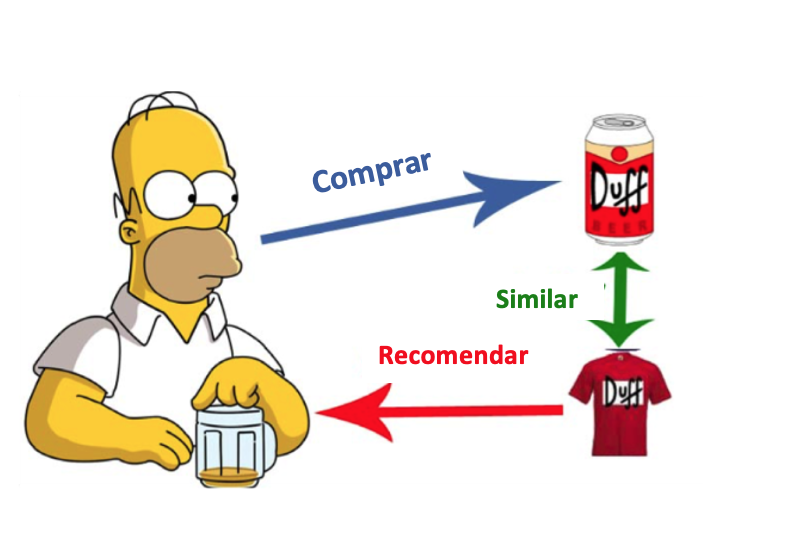
\includegraphics[scale=0.6]{../figs/Homero.png}
\end{figure}


\end{frame}    

%----------------------------------------------------------------------%
\begin{frame}
\frametitle{Filtrado colaborativo}
\framesubtitle{Basado en ítems}

\begin{figure}[H]
\centering

  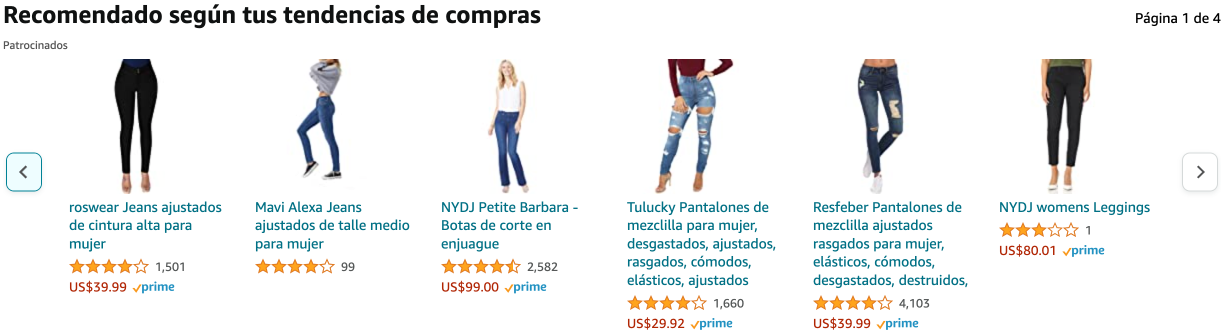
\includegraphics[scale=0.6]{../figs/item_jeans.png}
\end{figure}



\end{frame}    

%----------------------------------------------------------------------%
\begin{frame}
\frametitle{Filtrado colaborativo}
\framesubtitle{Basado en usuarios}

\begin{figure}[H]
\centering

  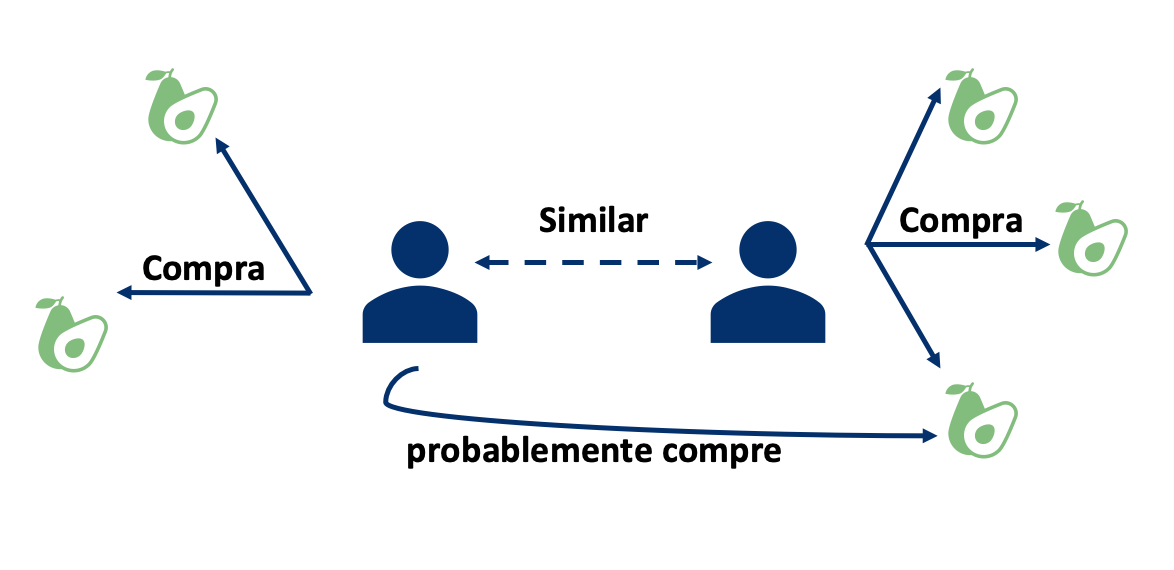
\includegraphics[scale=0.5]{../figs/aguacate.png}
\end{figure}



\end{frame}    
%----------------------------------------------------------------------%
\begin{frame}
\frametitle{Filtrado colaborativo}
\framesubtitle{Basado en ítems}

\begin{figure}[H]
\centering

  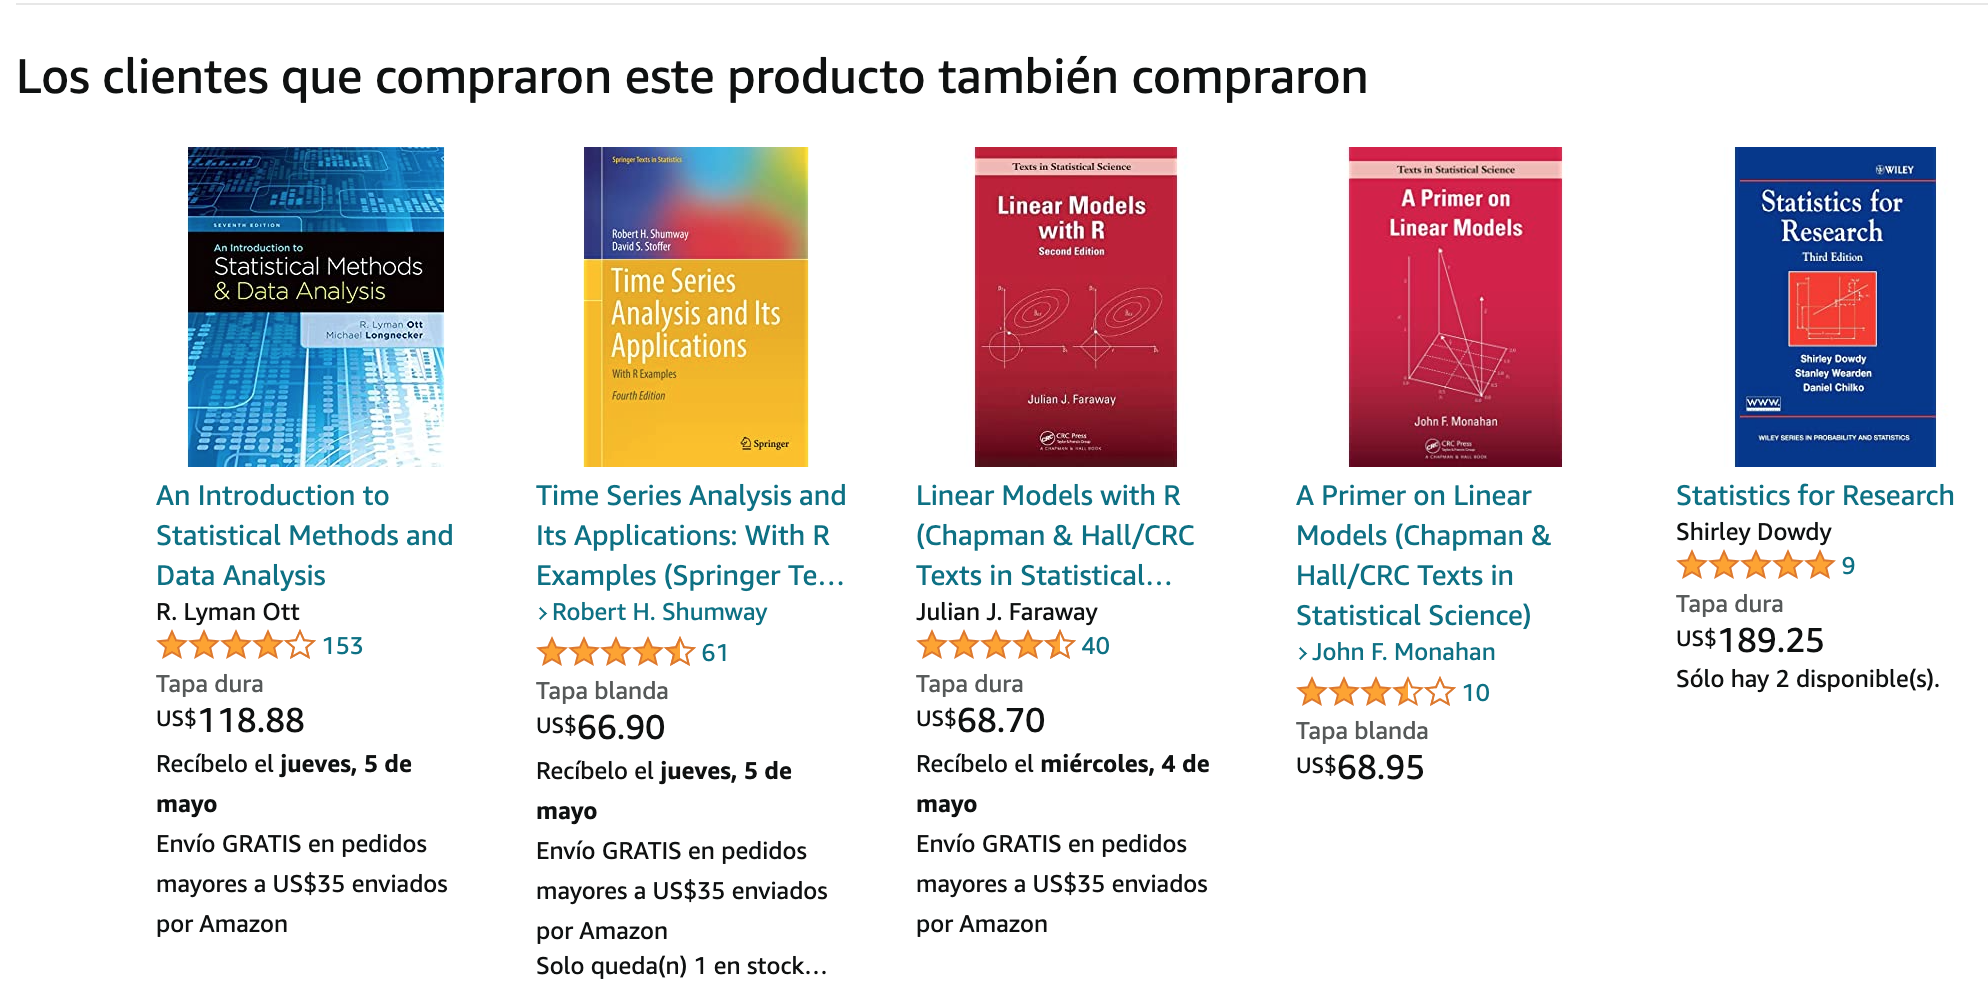
\includegraphics[scale=0.35]{../figs/usuario_libros.png}
\end{figure}


\end{frame}    
%----------------------------------------------------------------------%
\begin{frame}
\frametitle{Filtrado basado en contenido}

   
\begin{itemize}
 \item Estos sistemas brindan recomendaciones basadas en el perfil del usuario y  metadatos  sobre los artículos
 \end{itemize} 
 

    \begin{figure}[H]
\centering

  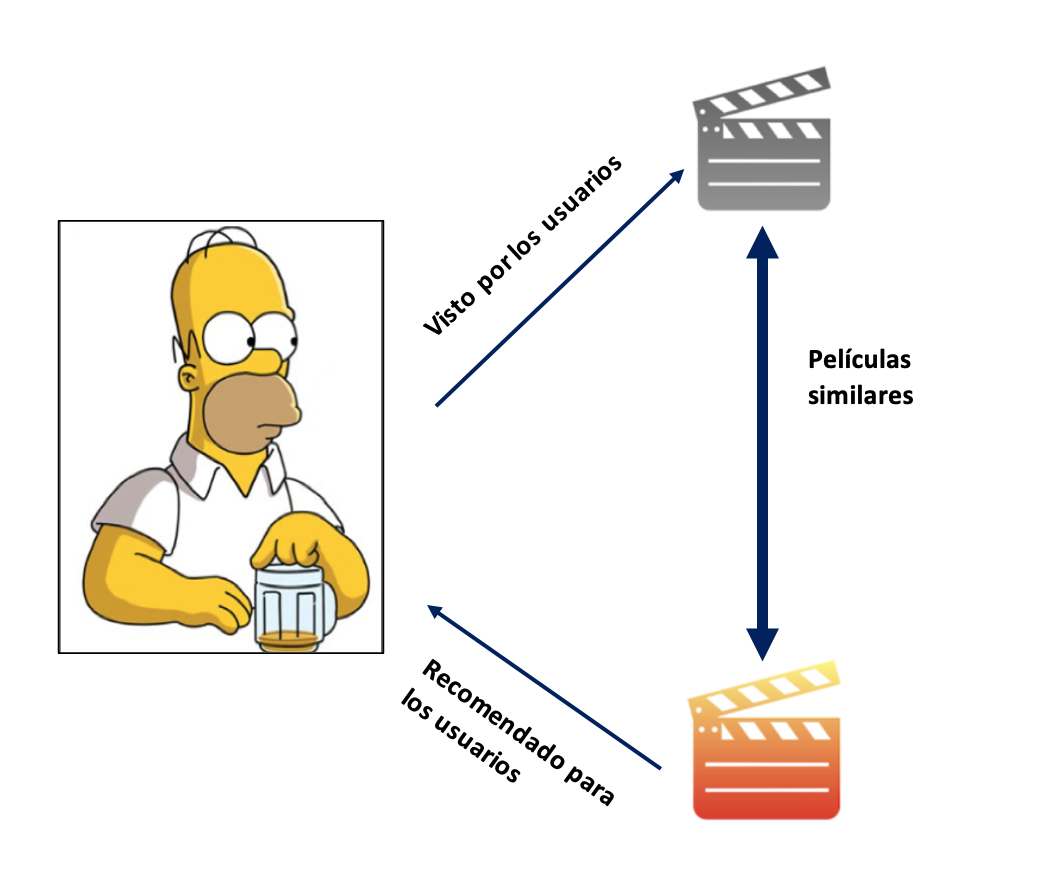
\includegraphics[scale=0.4]{../figs/Homero_movies.png}
\end{figure}

\end{frame}    
%----------------------------------------------------------------------%
\begin{frame}
\frametitle{Filtrado basado en contenido}
\framesubtitle{Basado en ítems}

\begin{figure}[H]
\centering

  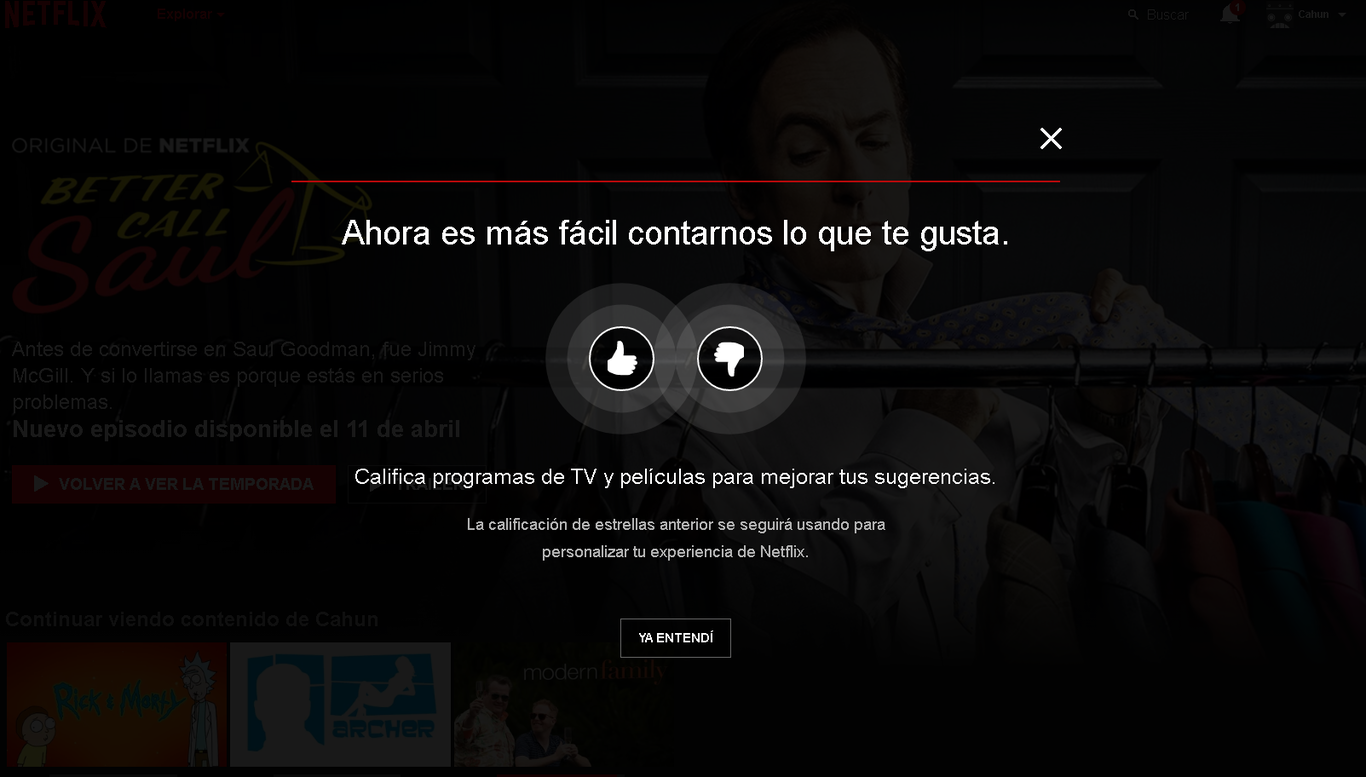
\includegraphics[scale=0.2]{../figs/netflix.png}
\end{figure}



\end{frame} 
%----------------------------------------------------------------------%
\begin{frame}
\frametitle{Recomendadores híbridos}

   
   \begin{itemize}
\item Estos son sistemas que combinan varios tipos de modelos de recomendación, superando así las deficiencias de cada uno.
\medskip
\item  Ejemplo: Netflix 
   \end{itemize}


   
\end{frame}    
    
%----------------------------------------------------------------------%

\section{Break}
\begin{frame}
\frametitle{}

\begin{centering}
\huge
\textcolor{andesred}{Volvemos en 10 min con \texttt{Python} }

\end{centering}

\end{frame}



    
%----------------------------------------------------------------------%
%----------------------------------------------------------------------%
\end{document}
%----------------------------------------------------------------------%
%----------------------------------------------------------------------%

